%% bare_conf_compsoc.tex
%% V1.4b
%% 2015/08/26
%% by Michael Shell
%% See:
%% http://www.michaelshell.org/
%% for current contact information.
%%
%% This is a skeleton file demonstrating the use of IEEEtran.cls
%% (requires IEEEtran.cls version 1.8b or later) with an IEEE Computer
%% Society conference paper.
%%
%% Support sites:
%% http://www.michaelshell.org/tex/ieeetran/
%% http://www.ctan.org/pkg/ieeetran
%% and
%% http://www.ieee.org/

%%*************************************************************************
%% Legal Notice:
%% This code is offered as-is without any warranty either expressed or
%% implied; without even the implied warranty of MERCHANTABILITY or
%% FITNESS FOR A PARTICULAR PURPOSE! 
%% User assumes all risk.
%% In no event shall the IEEE or any contributor to this code be liable for
%% any damages or losses, including, but not limited to, incidental,
%% consequential, or any other damages, resulting from the use or misuse
%% of any information contained here.
%%
%% All comments are the opinions of their respective authors and are not
%% necessarily endorsed by the IEEE.
%%
%% This work is distributed under the LaTeX Project Public License (LPPL)
%% ( http://www.latex-project.org/ ) version 1.3, and may be freely used,
%% distributed and modified. A copy of the LPPL, version 1.3, is included
%% in the base LaTeX documentation of all distributions of LaTeX released
%% 2003/12/01 or later.
%% Retain all contribution notices and credits.
%% ** Modified files should be clearly indicated as such, including  **
%% ** renaming them and changing author support contact information. **
%%*************************************************************************


% *** Authors should verify (and, if needed, correct) their LaTeX system  ***
% *** with the testflow diagnostic prior to trusting their LaTeX platform ***
% *** with production work. The IEEE's font choices and paper sizes can   ***
% *** trigger bugs that do not appear when using other class files.       ***                          ***
% The testflow support page is at:
% http://www.michaelshell.org/tex/testflow/



\documentclass[conference]{IEEEtran}
%\documentclass{IEEEtran}
% Some/most Computer Society conferences require the compsoc mode option,
% but others may want the standard conference format.
%
% If IEEEtran.cls has not been installed into the LaTeX system files,
% manually specify the path to it like:
% \documentclass[conference,compsoc]{../sty/IEEEtran}


%%%%%%%%%%%%%%%%%%%%%%%%%%%%%%%%%%%%%%%%%%%%%%%%%%%%%%%%%%
% Inline comments. Pick initials and color of your choice. \ysnote{} refers to Yogesh's note. 
%
\usepackage[usenames,dvipsnames,svgnames,x11names]{xcolor}
\newcommand{\ysnote}[1]{ {\textcolor{magenta} { ***Yogesh: #1 }}} % needs a response
\newcommand{\drnote}[1]{ {\textcolor{orange} { ***Dreamer: #1 }}}
\newcommand{\Note}[1]{\textcolor{red}{#1}} % verify if this is correct
\newcommand{\ysnoted}[1]{ {\textcolor{green} { ***TODO Later: #1 }}} % postpone addressing of comment

%%%%%%%%%%%%%%%%%%%%%%%%%%%%%%%%%%%%%%%%%%%%%%%%%%%%%%%%%%
% Additional fonts
\usepackage[T1]{fontenc} %% https://tex.stackexchange.com/questions/664/why-should-i-use-usepackaget1fontenc
\usepackage{lmodern} %% https://tex.stackexchange.com/questions/2369/why-do-the-less-than-symbol-and-the-greater-than-symbol-appear-wrong-as
\usepackage[normalem]{ulem} % required for strikeout font
% Default Computer Modern font (no bold implemented)
%\renewcommand{\ttdefault}{cmtt}
% Hence, Using Courier font
\renewcommand{\ttdefault}{pcr}


%%%%%%%%%%%%%%%%%%%%%%%%%%%%%%%%%%%%%%%%%%%%%%%%%%%%%%%%%%
% Change tracking for article revisions. Added, Deleted, Replaced, or Modified content.
%
\newcommand{\modc}[1]{{\textcolor{blue}{#1}}}
\newcommand{\addc}[1]{{\textcolor{teal}{#1}}}
\newcommand{\delc}[1]{ {\textcolor{gray} {\sout{#1}} }}
%\newcommand{\delc}[1]{} % uncomment this (and comment above line) to ignore showing deletion
\newcommand{\repc}[2]{ {\textcolor{gray} {\sout{#1}} }{\textcolor{teal} {#2}}}
%\newcommand{\repc}[2]{{\textcolor{teal}{#2}}} % uncomment this (and comment above line) to ignore showing deletion
%
%---------------------------------------------------------


%%%%%%%%%%%%%%%%%%%%%%%%%%%%%%%%%%%%%%%%%%%%%%%%%%%%%%%%%%
% *** MISC UTILITY PACKAGES ***
%
%\usepackage{ifpdf}
% Heiko Oberdiek's ifpdf.sty is very useful if you need conditional
% compilation based on whether the output is pdf or dvi.
% usage:
% \ifpdf
%   % pdf code
% \else
%   % dvi code
% \fi
% The latest version of ifpdf.sty can be obtained from:
% http://www.ctan.org/pkg/ifpdf
% Also, note that IEEEtran.cls V1.7 and later provides a builtin
% \ifCLASSINFOpdf conditional that works the same way.
% When switching from latex to pdflatex and vice-versa, the compiler may
% have to be run twice to clear warning/error messages.


%%%%%%%%%%%%%%%%%%%%%%%%%%%%%%%%%%%%%%%%%%%%%%%%%%%%%%%%%%
% *** CITATION PACKAGES ***
%
\usepackage[nocompress]{cite}
% cite.sty was written by Donald Arseneau
% V1.6 and later of IEEEtran pre-defines the format of the cite.sty package
% \cite{} output to follow that of the IEEE. Loading the cite package will
% result in citation numbers being automatically sorted and properly
% "compressed/ranged". e.g., [1], [9], [2], [7], [5], [6] without using
% cite.sty will become [1], [2], [5]--[7], [9] using cite.sty. cite.sty's
% \cite will automatically add leading space, if needed. Use cite.sty's
% noadjust option (cite.sty V3.8 and later) if you want to turn this off
% such as if a citation ever needs to be enclosed in parenthesis.
% cite.sty is already installed on most LaTeX systems. Be sure and use
% version 5.0 (2009-03-20) and later if using hyperref.sty.
% The latest version can be obtained at:
% http://www.ctan.org/pkg/cite
% The documentation is contained in the cite.sty file itself.
%
% Note that some packages require special options to format as the Computer
% Society requires. In particular, Computer Society  papers do not use
% compressed citation ranges as is done in typical IEEE papers
% (e.g., [1]-[4]). Instead, they list every citation separately in order
% (e.g., [1], [2], [3], [4]). To get the latter we need to load the cite
% package with the nocompress option which is supported by cite.sty v4.0
% and later.


%%%%%%%%%%%%%%%%%%%%%%%%%%%%%%%%%%%%%%%%%%%%%%%%%%%%%%%%%%
% When using XML fragments, using pretty-print is helpful.
%
\usepackage{listings}
% \usepackage{color}
% \definecolor{gray}{rgb}{0.4,0.4,0.4}
% \definecolor{darkblue}{rgb}{0.0,0.0,0.6}
%\definecolor{maroon}{rgb}{0.5,0,0}
% \definecolor{cyan}{rgb}{0.0,0.6,0.6}

\lstset{
  basicstyle=\ttfamily,
  columns=fullflexible,
  showstringspaces=false,
  commentstyle=\color{gray}\upshape,
  escapeinside={||},
  mathescape=true
}

\lstdefinelanguage{XML}
{
basicstyle=\ttfamily\footnotesize,
  morestring=[b]",
  moredelim=[s][\bfseries\color{Maroon}]{<}{\ },
  moredelim=[s][\bfseries\color{Maroon}]{</}{>},
  moredelim=[l][\bfseries\color{Maroon}]{/>},
  moredelim=[l][\bfseries\color{Maroon}]{>},
  morecomment=[s]{<?}{?>},
  morecomment=[s]{<!--}{-->},
  commentstyle=\color{gray},
  stringstyle=\color{blue},
  identifierstyle=\color{red}
%  morekeywords={type,id,value,impl}% list your attributes here
}
%
%---------------------------------------------------------


%%%%%%%%%%%%%%%%%%%%%%%%%%%%%%%%%%%%%%%%%%%%%%%%%%%%%%%%%%
% Better control over verbatim text
\usepackage{moreverb}

%%%%%%%%%%%%%%%%%%%%%%%%%%%%%%%%%%%%%%%%%%%%%%%%%%%%%%%%%%
% for syntax/grammar
\usepackage[nounderscore]{syntax}

%%%%%%%%%%%%%%%%%%%%%%%%%%%%%%%%%%%%%%%%%%%%%%%%%%%%%%%%%%
\usepackage[pdftex]{graphicx}
% declare the path(s) where your graphic files are
\graphicspath{{./figures/}}
% and their extensions so you won't have to specify these with
% every instance of \includegraphics
\DeclareGraphicsExtensions{.pdf}
% graphicx was written by David Carlisle and Sebastian Rahtz. It is
% required if you want graphics, photos, etc. graphicx.sty is already
% installed on most LaTeX systems. The latest version and documentation
% can be obtained at: 
% http://www.ctan.org/pkg/graphicx
% Another good source of documentation is "Using Imported Graphics in
% LaTeX2e" by Keith Reckdahl which can be found at:
% http://www.ctan.org/pkg/epslatex
%
% latex, and pdflatex in dvi mode, support graphics in encapsulated
% postscript (.eps) format. pdflatex in pdf mode supports graphics
% in .pdf, .jpeg, .png and .mps (metapost) formats. Users should ensure
% that all non-photo figures use a vector format (.eps, .pdf, .mps) and
% not a bitmapped formats (.jpeg, .png). The IEEE frowns on bitmapped formats
% which can result in "jaggedy"/blurry rendering of lines and letters as
% well as large increases in file sizes.
%
% You can find documentation about the pdfTeX application at:
% http://www.tug.org/applications/pdftex

% Definitions for placeholder figures
\newcommand{\dummyfigX}{\fbox{\parbox[h][1.75in][t]{0.95\textwidth}{\emph{Placeholder}}}} % full page width (figure*)
\newcommand{\dummyfigXX}{\fbox{\parbox[h][1.75in][t]{0.95\columnwidth}{\emph{Placeholder}}}} % 1 column width (in 2 column format)
\newcommand{\dummyfigXXX}{\fbox{\parbox[h][1.75in][t]{0.30\textwidth}{\emph{Placeholder}}}} % 1/3 full page width (figure*)
\newcommand{\dummyfigXXXX}{\fbox{\parbox[h][1.75in][t]{0.23\textwidth}{\emph{Placeholder}}}} % 1/4 full page width (figure*)


%%%%%%%%%%%%%%%%%%%%%%%%%%%%%%%%%%%%%%%%%%%%%%%%%%%%
% *** MATH PACKAGES ***
%
\usepackage[cmex10]{amsmath}
\usepackage{amssymb}
\usepackage{mathtools}
\usepackage{amsthm}
\usepackage{amsfonts}
\newtheorem{cons}{Constraint}
%
% A popular package from the American Mathematical Society that provides
% many useful and powerful commands for dealing with mathematics.
%
% Note that the amsmath package sets \interdisplaylinepenalty to 10000
% thus preventing page breaks from occurring within multiline equations. Use:
%\interdisplaylinepenalty=2500
% after loading amsmath to restore such page breaks as IEEEtran.cls normally
% does. amsmath.sty is already installed on most LaTeX systems. The latest
% version and documentation can be obtained at:
% http://www.ctan.org/pkg/amsmath



%%%%%%%%%%%%%%%%%%%%%%%%%%%%%%%%%%%%%%%%%%%%%%%%%%%%
% *** SUBFIGURE PACKAGES ***
\usepackage{subfig} %[caption=false,font=footnotesize,labelfont=sf,textfont=sf]
%
% subfig.sty, written by Steven Douglas Cochran, is the modern replacement
% for subfigure.sty, the latter of which is no longer maintained and is
% incompatible with some LaTeX packages including fixltx2e. However,
% subfig.sty requires and automatically loads Axel Sommerfeldt's caption.sty
% which will override IEEEtran.cls' handling of captions and this will result
% in non-IEEE style figure/table captions. To prevent this problem, be sure
% and invoke subfig.sty's "caption=false" package option (available since
% subfig.sty version 1.3, 2005/06/28) as this is will preserve IEEEtran.cls
% handling of captions.
% Note that the Computer Society format requires a sans serif font rather
% than the serif font used in traditional IEEE formatting and thus the need
% to invoke different subfig.sty package options depending on whether
% compsoc mode has been enabled.
%
% The latest version and documentation of subfig.sty can be obtained at:
% http://www.ctan.org/pkg/subfig




% *** SPECIALIZED LIST PACKAGES ***
%
\usepackage{algorithmicx}
\usepackage{algpseudocode}
\usepackage[ruled]{algorithm}
\definecolor{light-gray}{gray}{0.75}
\algrenewcommand{\algorithmiccomment}[1]{\hskip3em{{\footnotesize \textcolor{light-gray}{$\blacktriangleright$}}} #1}
%
% This package provides an algorithmic environment fo describing algorithms.
% You can use the algorithmic environment in-text or within a figure
% environment to provide for a floating algorithm. 


%%%%%%%%%%%%%%%%%%%%%%%%%%%%%%%%%%%%%%%%%%%%%%%%%%%%%%%%%%
% Table relates packages
\usepackage{multirow} % Multi-row tables
\usepackage{rotating} % sideways table
\usepackage{booktabs} % better lines
\usepackage{colortbl} % cell colors
\usepackage{tablefootnote} % add support for footnote in table

%%%%%%%%%%%%%%%%%%%%%%%%%%%%%%%%%%%%%%%%%%%%%%%%%%%%%%%%%%
% *** PDF, URL AND HYPERLINK PACKAGES ***
%
%\usepackage[colorlinks,bookmarksopen,bookmarksnumbered,citecolor=red,urlcolor=red]{hyperref}
\usepackage[pdftex,colorlinks=true,urlcolor=blue,citecolor=blue]{hyperref}


%%%%%%%%%%%%%%%%%%%%%%%%%%%%%%%%%%%%%%%%%%%%%%%%%%%%%%%%%%
% Avoids contiguous empty spaces
\usepackage{xspace}

%%%%%%%%%%%%%%%%%%%%%%%%%%%%%%%%%%%%%%%%%%%%%%%%%%%%%%%%%%
% IEEETrans class fix for enumitem. provide for legacy IED commands/lengths when possible
% http://comments.gmane.org/gmane.editors.lyx.general/68611
\let\labelindent\relax
\usepackage{enumitem}


%%%%%%%%%%%%%%%%%%%%%%%%%%%%%%%%%%%%%%%%%%%%%%%%%%%%%%%%%%
% correct bad hyphenation here
\hyphenation{compu-ta-tio-nal}

% define repetitive complex fragments here
\newcommand{\floe}{$\mathcal{F}{\ell}{o}{\varepsilon}$\xspace}
\newcommand{\prc}{\mathcal{P}}
\newcommand{\chn}{\mathcal{C}}


%%%%%%%%%%%%%%%%%%%%%%%%%%%%%%%%%%%%%%%%%%%%%%%%%%%%%%%%%%
% generate lorum ipsum placeholder text
%\usepackage[english]{babel}
\usepackage{blindtext}
\newcommand{\blindtextc}{\color{gray}\blindtext\color{black}}
\newcommand{\Blindtextc}{\color{gray}\Blindtext\color{black}}




\begin{document}

\title{Distributed Knowledge Graph Querying on \\ Edge and Cloud}


\author{\IEEEauthorblockN{Shriram R.}\\
\IEEEauthorblockA{Department of Computational and Data Sciences\\
Indian Institute of Science, Bangalore 560012 INDIA\\
Email: shriramr@iisc.ac.in}
}


\maketitle


\begin{abstract}
In this mid-term period, a basic distributed knowledge graph querying system has been implemented by adopting an existing graph database engine with functionalities to fetch and store local knowledge graph, partition queries for local and remote graph database, combining results from local and remote for vertex search, edge search and shortest path search queries. Experiments were performed using a small dataset to study the performance of different types of queries and an analysis of result has been performed.  
\end{abstract}

\section{System Design and Implementation}

The following sections cover the system design and implementation completed so far with respect to the proposed targets for midterm,

\subsection{Remote (Cloud) Layer}
This layer consists of an in-memory graph database engine \emph{Tinkergraph} running on the head node of \emph{Rigel} Cluster. Integration of GoDB was explored but due to technical issues, \emph{Tinkergraph} was chosen as the desired engine. It offers a good set of APIs to run a variety of queries related to graphs and supports different programming languages. A distributed version spanning multiple nodes will be explored in future.

\subsection{Edge Layer}
The edge layer consists of different modules each with a specific functionality. The modules are explained in detail in the section below,

\subsubsection{Edge Graph Processing}
The same \emph{tinkergraph} engine used in the remote layer is spawned on the edge as a single node in-memory store. The performance of this is evaluated through experiments. A custom engine is required only if the edge based \emph{tinkergraph} engine is found to be a bottleneck.

\subsubsection{Knowledge Graph Partitioning}
The logic for partitioning is based on the association of an edge with a single entity in the Knowledge graph. E.g. <India>. Given a entity, this module queries the remote server to fetch the subgraph centered at the given entity and spanning for a specified number of hops (E.g. 2). This subgraph is then inserted into the \emph{Tinkergraph} server running locally and forms the local knowledge graph.

\subsubsection{Query Partitioning}
The query partitioning module divides the input query into local and remote queries and fires them against the respective servers. The input queries are provided in JSON format with custom fields for each query type. The logic is different for each type of query. It is detailed below,
\begin{itemize}%[noitemsep,topsep=0pt,parsep=0pt,partopsep=0pt]
	\item \emph{Vertex Search} - The given query consists of three fields one for label based search, one for set of vertices with incoming edge from a given vertex and one for set of vertices with outgoing edge to a given vertex. The query is unmodified and used for local and remote since this search operation is embarrassingly parallel
	\item \emph{Edge Search} - The given query is unmodified as in the previous case since it also embarrassingly parallel and consists of three fields one for label based search, one for all edges outgoing from a vertex and other for all edges incoming to a vertex
	\item \emph{Path Search} - The path search queries consists of a source vertex and target vertex and finds the shortest path between them in an undirected knowledge graph. It can have three result types: Full path is in edge layer, full path is in remote layer and path crosses edge and remote layer. The logic follows these steps,
	\begin{itemize}
		\item A local query is fired first to search for path completely contained in the edge layer
		\item If the previous step returns no path, then a series of queries are fired to the remote layer with source vertex changed to \emph{cut vertices} and target vertex unchanged. This will return a portion of shortest path in the remote server
		\item A series of local queries are fired to determine the paths from original source to \emph{cut vertices}. 
	\end{itemize}
\end{itemize}

\subsubsection{Combining Query Results}
Combining the query results is implemented as follows,
\begin{itemize}
	\item \emph{Vertex \& Edge Search} - The result set from local and remote server search are combined using \emph{set union} operation
	\item \emph{Path search} - If the path is entirely contained inside edge, the local server result is directly used. For cross paths, The result from local server and remote server are joined at the \emph{cut vertex} and then the shortest path is determined and provided as output
\end{itemize}

 

%\begin{figure*}[th]
%	\centering%~%
%	\subfloat[High Level Architecture]{
%		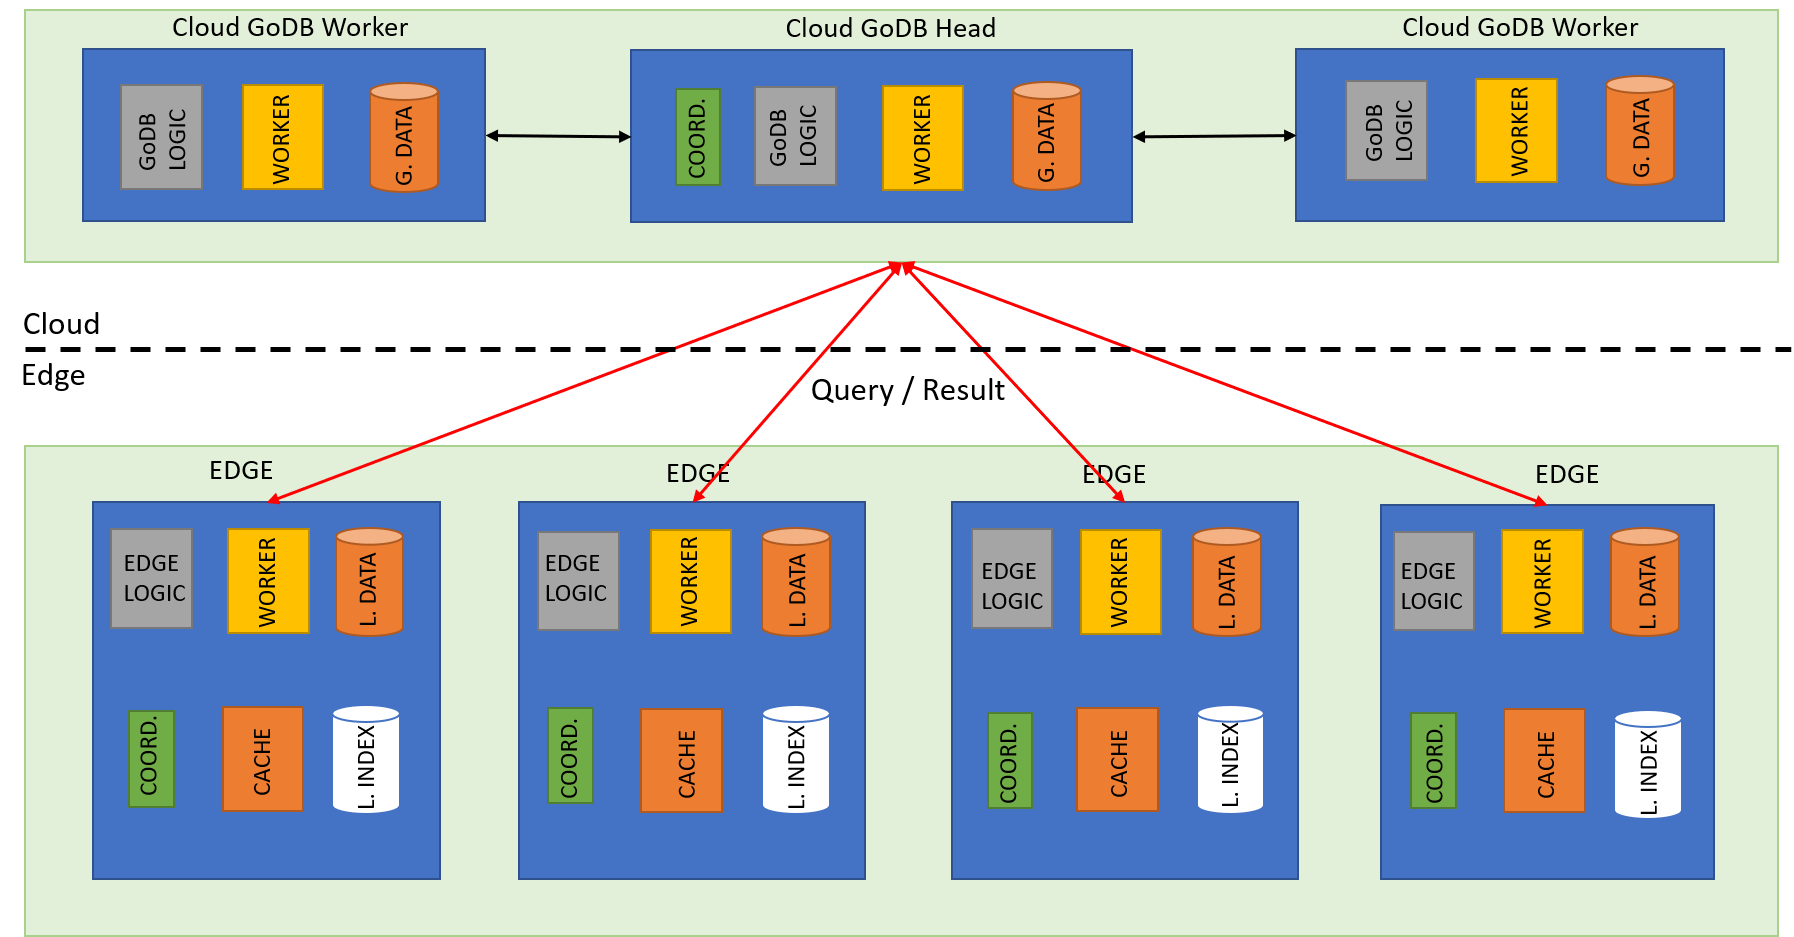
\includegraphics[height=0.23\textheight]{5.png}
%		\label{fig:arch}
%	}\qquad
%	\subfloat[Logical Flow]{
%		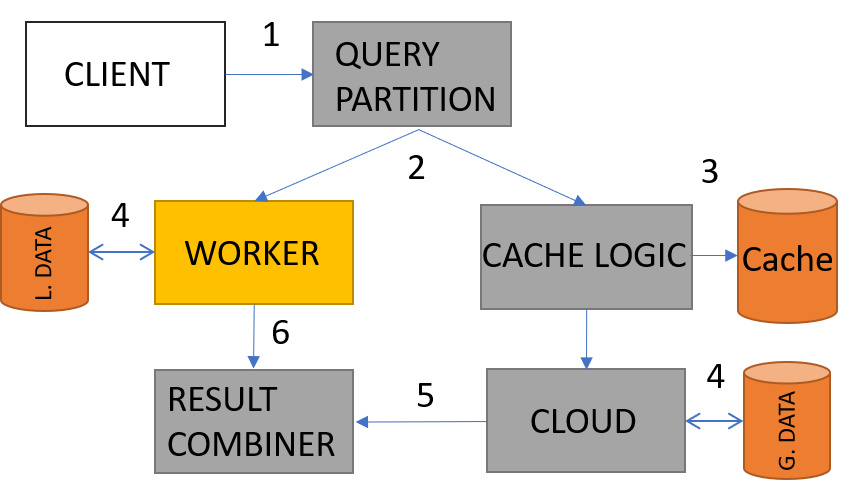
\includegraphics[height=0.15\textheight]{6.png}
%		\label{fig:logic-flow}
%	}\\
%	\label{fig:problem-approach}
%	\caption{Proposed Design}
%	\vspace{-0.1in}
%\end{figure*} 


\section{Experiments}

The experimental setup is as follows: Microsoft Azure cloud platform will be used to run the entire edge-cloud setup. 5 D4 VMs will be used to run the cloud layer. These VMs will host the GoDB head and worker nodes. GoDB uses GoFFish v2.6 and Java v1.7. VIoLET\cite{DBLP:journals/corr/abs-1806-06032} will be used to virtually emulate the entire edge layer. 20 edges of type Pi3B+ will be created and interconnected with each other. The latency and bandwidth of edge-edge and edge-cloud will be set to 1ms-50mbps and 5ms-20mbps respectively. All the devices will be running on CentOS v7.

The YAGO dataset will be the primary knowledge graph data that will be used for the experiments. Since the size of the full dataset is huge, only a fraction of the dataset will be potentially used based on the availability of sufficient cloud resources. NELL\cite{Mitchell:2018:NL:3210350.3191513} could be used as a secondary dataset. The baseline system for comparison will be GoDB in cloud layer with all the edges running all the queries directly on the cloud without caching. The graph in GoDB will be partitioned using METIS with one subgraph per core.

The query workload for the experiments will be of the following types - Vertex search, Edge search, Reachability, Neighbourhood, Shortest Path and as a stretch goal, Subgraph Isomorphism. 

The size of the knowledge graph that be accommodated inside the edge device will be determined through the following experiment - 10 queries of each type will be triggered on the edge for different sizes of local graph which is doubled in each iteration. The same set of query will also be triggered in cloud and the time taken in both the cases will be measured. This size should be the maximum size in which the local query time is less than the global query time for the same subgraph. This size will be used in all the below experiments as well.

\textbf{Microbenchmarks}
\begin{enumerate}%[noitemsep,topsep=0pt,parsep=0pt,partopsep=0pt]
	\item Query partitioning logic will incur some time to partition the query and generate a query plan. It is useful to measure this time for each query type. An experiment is performed with 100 different queries for each type being run on the edge and the time to partition is measured and plotted as a violin plot. The violin should ideally not have long tails.
	\item Graph indexing time and memory has to be measured for different query types as a function of graph size. In this experiment, for each graph size, index construction time and index size is measured for each index type. The time taken and size should increase as per the time and space complexity of the index.
\end{enumerate}

The experiments will test the impact of query partitioning, query caching and graph indexing. The key metric to be measured is the query latency (time to get the results).  

\begin{enumerate}%[noitemsep,topsep=0pt,parsep=0pt,partopsep=0pt]
	\item \textbf{Query Partitioning:} 100 random queries of each type will be triggered in total with the queries uniformly and randomly distributed across all the edges. The time taken to complete the query in the local knowledge graph, the global knowledge graph and query completion time is measured. When compared with baseline, the query completion time should be less in the new system and the local querying time should be far less than the global time since the size of local graph will be smaller compared to the global graph. This showcases the effectiveness of Query Partitioning on the performance.
    \item \textbf{Query Caching:} There will be two baselines for comparison. One is the cloud only baseline and the other is the edge-cloud setup with cache disabled. In this experiment, each edge will have 20 different queries. These queries will be executed 5 times each in random order. This is to enable repetition of the same query from a given edge device. The time taken to complete the query in local and global graph and the total time will be measured. The cache hit/miss count will also be logged for each query execution. The cache enabled version should ideally outperform the other two baselines in terms of global execution time since the global query result will be cached in the edge.
    \item \textbf{Graph Indexing:} The baseline for graph indexing will be edge-cloud setup with indexing disabled on the edge. This experiment consists of 100 random queries of each type similar to the Query Partitioning experiment. The time taken to complete the local query with index and without index is measured. The outcome should be that the time taken with index should be less than the without index baseline. The effectiveness of each index for each query type will be different since problems which are NP complete like subgraph isomorphism will offer more benefit in having the index than other simple problems like vertex or edge search.
\end{enumerate}

% trigger a \newpage just before the given reference
% number - used to balance the columns on the last page
% adjust value as needed - may need to be readjusted if
% the document is modified later
%\IEEEtriggeratref{6}
% The "triggered" command can be changed if desired:
%\IEEEtriggercmd{\enlargethispage{-5in}}

% references section

% can use a bibliography generated by BibTeX as a .bbl file
% BibTeX documentation can be easily obtained at:
% http://mirror.ctan.org/biblio/bibtex/contrib/doc/
% The IEEEtran BibTeX style support page is at:
% http://www.michaelshell.org/tex/ieeetran/bibtex/
\bibliographystyle{IEEEtran}
% argument is your BibTeX string definitions and bibliography database(s)
\bibliography{paper}

% that's all folks
\end{document}

%%% Local Variables:
%%% mode: latex
%%% TeX-master: t
%%% End:
